\chapter{(Linear) Group Actions}


If $G$ is a group then we denote by $e \in G$ the neutral element and by $gh$ the composition of $g,h \in G$ and by $g^{-1}$ the inverse of $g \in G$.


\begin{defi}
 Given a group $G$ and a set $X$ then an action of $G$ on $X$ is a map
 \[
  \pi : G \times X \to X, (g,x) \to g.x,
 \]
 such that
 \begin{gather*}
  e.x = x \text{ and }
  (gh).x = g.(h.x)
 \end{gather*}
 for all $x \in X, g,h \in G$. We say then that $X$ is a $G$-set.
\end{defi}


\begin{defi}
 Given a set $X$ let
 \[
  S(X) := \{f : X \to X | f \text{ is bijective}\}.
 \]
 $S(X)$ is then a group with $fg := f \circ g$ (composition of maps) for all $f,g \in S(X)$ and $e = \id_X$.
\end{defi}


Given a group action $\pi : G \times X \to X$ any  $g \in G$ defines $\pi_g \in S(X)$ by setting
\[
 \pi_g(x) = \pi(g.x) \text{ for all } x \in X, g \in G.
\]


\begin{lem}
 Fix $G$ a group, $X$ a set. Then there is a 1:1-correspondence
 \[
 \begin{matrix}
    \left\{\text{$G$-actions on $X$}\right\}
  & \overset{1:1}{\longleftrightarrow}
  & \left\{\text{group homomorphisms $G \to S(X)$}\right\} \\
    \pi
  & \longmapsto
  & \hat{\pi} \\
    \mathring{\varphi}
  & \longmapsfrom
  & \varphi
  \end{matrix}
 \]
 where
 \[
  \hat{\pi}(g)(x) = g.x \text{ and } \mathring{\varphi}((g,x)) = \varphi(g)(x)
 \]
 for all $x \in X, g \in G$.
\end{lem}


From this Lemma we get the idea that group actions are ``the same'' as ``representing'' groups as permutation groups.


\begin{expl}
 Let $G$ be a group.
 \begin{enumerate}
  \item
   $G$ acts on itself by left multiplication, i.e.
   \[
    g.x = gx \text{ for all } g \in G, x \in X=G.
   \]
   This is called the \emph{(left) regular action of $G$}.
  \item
   $G$ acts onto itself by right multiplication with the inverse, i.e
   \[
    g.x = xg^{-1} \text{ for all } g \in G, x \in X=G.
   \]
   This is called the \emph{right regular action}.
  \item
   $G$ acts onto itself by conjugation, i.e.
   \[
    g.x = gxg^{-1} \text{ for all }g \in G, x \in X=G.
   \]
  \item
   Let $X$ be any set. Then $g.x = x$ for all $g \in G, x \in X$ defines an action. This is called the \emph{trivial action} and $X$ is called a \emph{trivial $G$-set}.
  \item
   Let $X, Y$ be $G$-sets. Then
   \[
    \Maps(X,Y) = \{f | f : X \to Y\}
   \]
   is a $G$-set by setting
   \[
    (g.f)(x) = g.\left(f\left(g^{-1}.x\right)\right)
   \]
   for all $g \in G, x \in X$.
   In the special case that $Y$ is a trivial $G$-set this means $(g.f)(x) = f(g^{-1}.x)$ for all $g \in G, x \in X$.
  \item
   If $X, Y$ are $G$-sets then $X \times Y$ is a $G$-set via
   \[
    g.(x,y) = (g.x,g.y) \text{ for all } g \in G, x \in X, y \in Y.
   \]
  \item
   If $X$ is a set and $G = S(X)$, then $X$ is a $G$-set via $f.x = f(x)$ for all $f \in G, x \in X$.
 \end{enumerate}
\end{expl}


\begin{defi}
 Let $G$ be a group and $X, Y$ $G$-sets. Then $f : X \to Y$ is called G-equivalent if
 \[
  f(g.x) = g.f(x)
 \]
 for all $g \in G, x \in X$. Denote
 \[
  \Hom_G(X,Y) = \{f : X \to Y | f \text{ is $G$-equivalent}\}.
 \]
\end{defi}


\begin{lem}
 Let $G$ be a group.
 \begin{enumerate}
  \item If $X$ is a $G$-set, then $\id_X \in \Hom_G(X,X)$.
  \item If $X, Y, Z$ are $G$-sets with $f_1 \in \Hom_G(X,Y)$ and $f_2 \in \Hom_G(Y,Z)$ then $f_2 \circ f_1 \in \Hom_G(X,Z)$.
 \end{enumerate}
\end{lem}


\begin{expl}
 \begin{enumerate}
  \item
   Let $G$ be a group and look at $G$ as a regular $G$-set. Then $f : G \to G$ is $G$-equivalent if and only if $f$ is given by right multiplication with some element $a \in G$ (i.e $f(g) = ga$ for all $g \in G$).
   \begin{proof}
    Assume there exists $a \in G$ such that $f(g) = ga$ for all $g \in G$. Then
    \[
     f(g.x) = f(gx) = (gx)a = g(xa) = g.f(x)
    \]
    for all $g, x \in G$. To show the other direction set $a := f(e)$. Because $f$ is $G$-equivalent we then have
    \[
     f(g) = f(ge) = f(g.e) = g.f(e) = g.a = ga
    \]
    for all $g \in G$.
   \end{proof}
  \item
   If $X$ and $Y$ are trivial $G$-sets then $\Hom_G(X,Y) = \Maps(X,Y)$.
  \item
   If $X$ is a $G$-set and $Y$ is a trivial $G$-set then
   \[
    \Hom_G(X,Y) = \{f : X \to Y | f(g.x) = f(x) \text{ for all } g \in G, x \in X\}.
   \]
 \end{enumerate}
\end{expl}


\begin{defi}
 Let $X$ be a $G$-set. We write
 \[
  X/G := \{\text{orbits of $G$ in $X$}\}.
 \]
\end{defi}


\begin{note}
 There is an induced, but trivial action of $G$ on $X/G$ from the action of $G$ on $X$, and the canonical map
 \[
  \can : X \to X/G, x \mapsto \text{orbit of } x
 \]
 is $G$-equivalent, since
 \[
  \can(g.x) = \text{orbit of $g.x$} = \text{orbit of $x$} = \can(x) = g.\can(x)
 \]
 for all $g \in G, x \in X$.
\end{note}


\begin{defi}
 Let $X$ be a $G$-set. Then
 \[
  X^G := \{\text{$G$-invariants of $X$}\} = \{x \in X : g.x = x \text{ for all } g \in G\}.
 \]
 The elements in $X^G$ are called $G$-invariants or $G$ fix points.
\end{defi}


\begin{lem}
 Let $X, Y$ be $G$-sets. Then $\Hom_G(X,Y) = \Maps(X,Y)^G$.
\end{lem}
\begin{proof}
 \begin{align*}
  f \in \Hom_G(X,Y)
  &\Leftrightarrow \forall g \in G, x \in X : f(g.x) = g.f(x) \\
  &\Leftrightarrow \forall g \in G, x \in X : f(g^{-1}.x) = g^{-1}.f(x) \\
  &\Leftrightarrow \forall g \in G, x \in X : g.f(g^{-1}.x) = f(x) \\
  &\Leftrightarrow \forall g \in G : g.f = f \\
  &\Leftrightarrow f \in \Maps(X,Y)^G.
 \end{align*}
\end{proof}


\begin{defi}
 Let $X$ be a $G$-set, $k$ a field or a ring. $f : X \to k$ is called invariant (or better $G$-invariant) if
 \[
  f(x) = f(g^{-1}.x) \text{ for all } g \in G, x \in X.
 \]
\end{defi}


\begin{note}
 This agrees with the above definition of $f \in \Hom_G(X,k) = \Maps(X,k)^G$ if we consider $k$ as a trivial $G$-set.
\end{note}


\begin{lem}
 Let $X$ be a $G$-set, $k$ a field or a ring. Then $f : X \to k$ is invariant if and only if $f$ factors through $\can$, i.e. if the following diagram commutes.
 \begin{center}
 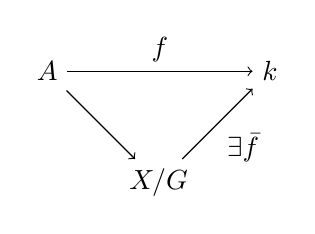
\begin{tikzpicture}[node distance = 2cm, auto]
  \node (A) {$A$};
  \node (XG) [below right of = A] {$X/G$};
  \node (k) [above right of = XG] {$k$};
  \draw[->] (A) to node {$f$} (k);
  \draw[->] (A) to node [swap] {$\can$} (XG);
  \draw[->] (XG) to node [swap] {$\exists\bar{f}$} (k);
 \end{tikzpicture}
 \end{center}
\end{lem}
\begin{proof}
 If $f$ is invariant then $f(x) = f(g^{-1}.x)$ for all $g \in G, x \in X$. Therefore $f$ is constant on orbits. Now define $\bar{f}(\mc{O}) = f(x)$ where $\mc{O}$ is an orbit and $x \in \mc{O}$.
 
 To show the other direction assume $f$ factors through $\can$. Then $f$ is constant on orbits, i.e. $f(x) = f(g.x)$ for all $g \in G, x \in X$, i.e. $f(x) = f(g^{-1}.x)$ for all $g \in G, x \in X$. Therefore $f$ is invariant.
\end{proof}












